\documentclass[conference]{IEEEtran}

% Pacotes para suporte ao Português e imagens
\usepackage[utf8]{inputenc}
\usepackage[T1]{fontenc}
\usepackage[brazilian]{babel}
\usepackage{amsmath,amssymb,amsfonts}
\usepackage{algorithmic}
\usepackage{graphicx}
\usepackage{textcomp}
\usepackage{xcolor}

\begin{document}

\title{Relatório de Práticas em Sistemas Digitais - Laboratório 05}

\author{\IEEEauthorblockN{Lucca Dultra, João Vital, Danye, Franksteps}
\IEEEauthorblockA{\textit{Departamento de Computação (DCOMP)} \\
\textit{Universidade Federal de Sergipe (UFS)}\\
São Cristóvão, Brasil \\
}
}

\maketitle

\begin{abstract}
Este relatório descreve as atividades do Laboratório 05, que introduz a simulação de circuitos utilizando o simulador NGSpice em conjunto com uma biblioteca de células comerciais padrão (Nangate FreePDK45 em 45nm). O estudo avalia a relação entre as dimensões físicas das células lógicas e seus impactos no desempenho e na dissipação de potência dinâmica. Através da síntese de um Multiplexador 2:1, analisa-se como o escalonamento do \textit{drive strength} (X1 para X2) influencia os picos de corrente no chaveamento capacitivo. Além disso, discute-se teoricamente a vantagem térmica e em área das células complexas (AOI) em relação às portas discretas equivalentes.
\end{abstract}

\begin{IEEEkeywords}
NGSpice, CMOS, Nangate 45nm, Consumo Dinâmico, Multiplexador, Células Padrão.
\end{IEEEkeywords}

\section{Introdução Teórica}
Nos fluxos modernos de projeto em microeletrônica, circuitos digitais complexos raramente são construídos desenhando-se transistores individuais. Ao invés disso, os engenheiros utilizam as \textit{Standard Cell Libraries} (Bibliotecas de Células Padrão). Estas bibliotecas fornecem portas lógicas pré-caracterizadas em diferentes dimensões e forças de condução (\textit{drive strengths}, como X1, X2, X4). 

Embora células maiores possam carregar redes capacitivas mais rapidamente e reduzir o tempo de transição de um sinal, elas não são isentas de custos. O escalonamento da dimensão do transistor aumenta as áreas de difusão e porta, o que eleva a capacitância parasita intrínseca do dispositivo. Como o consumo dinâmico na tecnologia CMOS está diretamente atrelado à carga e descarga dessas capacitâncias parasitas, circuitos mais robustos energeticamente dissipam mais potência térmica e exigem picos de corrente mais elevados, evidenciando o constante compromisso (\textit{trade-off}) no design de circuitos integrados.

\section{Materiais Utilizados}
\begin{itemize}
    \item Simulador de circuitos NGSpice.
    \item Design Kit Preditivo da NCSU para 45nm (FreePDK45).
    \item Biblioteca de células padrão da Nangate para o FreePDK45 (Tensão de alimentação $V_{DD} = 1.1\text{V}$).
\end{itemize}

\section{Descrição das Atividades e Resultados}

\subsection{Ambientação com a Sintaxe da Biblioteca (Ativ. 00 e 01)}
A prática inicial consistiu em executar \textit{netlists} pré-configuradas no NGSpice para testar portas inversoras. Ao simular inversores com capacidades geométricas diferentes (\texttt{INV\_X1}, \texttt{INV\_X2} e \texttt{INV\_X4}), verificou-se no gráfico transiente que as saídas apresentam comportamentos distintos em relação ao atraso (Fig. \ref{fig1}). 

Esse fenômeno ocorre porque células com maiores dimensões (como a X4) possuem canais mais largos, o que reduz drasticamente a resistência de condução dos transistores em comparação às células menores (X1). Essa menor resistência permite fornecer mais corrente em menos tempo, tornando o chaveamento (tempos de subida e descida) muito mais íngreme e rápido.

\begin{figure}[htbp]
\centerline{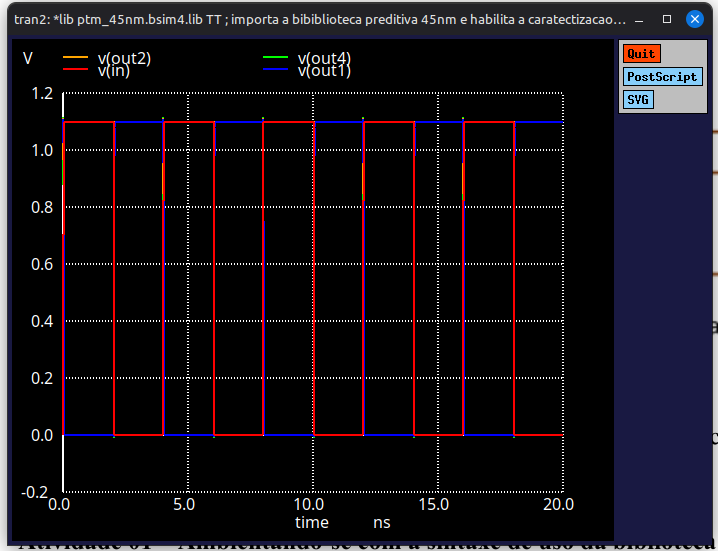
\includegraphics[width=\columnwidth]{1.png}}
\caption{Resposta transiente demonstrando as diferentes transições de inversores X1, X2 e X4.}
\label{fig1}
\end{figure}

\subsection{Circuito Multiplexador e Simulação (Atividade 02)}
Avançando no uso da biblioteca Nangate, foi descrito o arquivo \texttt{mux.sp} implementando um Multiplexador 2:1 composto por uma porta \texttt{INV\_X1}, duas portas \texttt{AND2\_X1} e uma porta \texttt{OR2\_X1}, possuindo um capacitor de carga de 10fF em série com a saída. 

Para extrair os fenômenos operacionais, os sinais de entrada de dados foram fixados em lógica antagônica ($\text{IN2} = 1$ e $\text{IN1} = 0$), e o sinal de Seleção (\text{SEL}) foi configurado como um gerador de pulso oscilando a uma frequência de 50 MHz (período de 20 ns). Na Figura \ref{fig2}, observa-se a correta seleção do circuito, e constata-se a geração pontual de picos de corrente ocorrendo estritamente durante os instantes em que o seletor comuta.

\begin{figure}[htbp]
\centerline{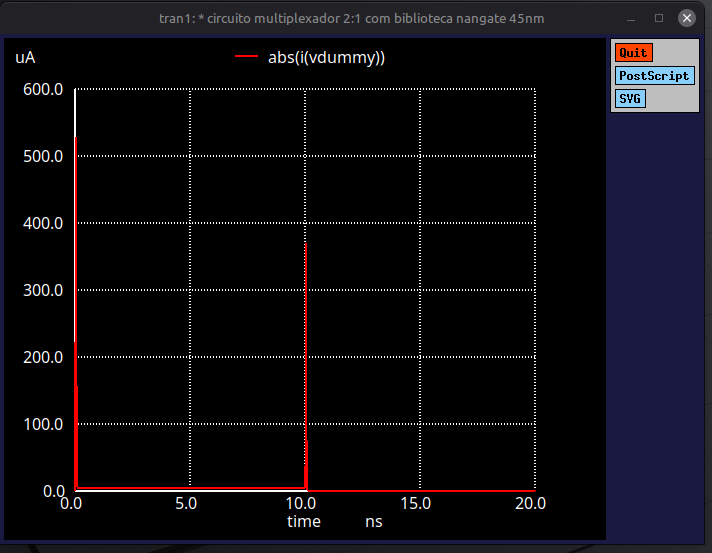
\includegraphics[width=\columnwidth]{2.png}}
\caption{Sinais de entrada, resposta lógica do MUX na saída e os picos de corrente instantânea para a tecnologia X1.}
\label{fig2}
\end{figure}

\subsection{Análise de Potência e Escalonamento Geométrico}
Através dos comandos de medição (comando \texttt{meas}) do próprio NGSpice, foi extraída a corrente média exata fornecida pela fonte no intervalo da simulação de um período (de 0 a 20 ns). A potência dissipada dinamicamente foi obtida pela equação $P = V_{DD} \cdot I_{med}$. 

Na primeira execução, utilizando unicamente células de dimensão **1X**, obteve-se:
\begin{itemize}
    \item \textbf{Corrente média ($I_{med1X}$):} $3,91 \mu A$
    \item \textbf{Potência Dissipada:} $P = 1.1\text{V} \times 3,91 \mu A \approx 4,30 \mu W$
\end{itemize}

Em seguida, os parâmetros do arquivo foram alterados para que todas as instâncias utilizassem células de dimensão **2X** (\texttt{INV\_X2}, \texttt{AND2\_X2}, \texttt{OR2\_X2}). O novo teste acusou um aumento expressivo no consumo (Fig. \ref{fig3}):
\begin{itemize}
    \item \textbf{Corrente média ($I_{med2X}$):} $9,77 \mu A$
    \item \textbf{Potência Dissipada:} $P = 1.1\text{V} \times 9,77 \mu A \approx 10,75 \mu W$
\end{itemize}

O consumo de energia mais que dobrou. Isso ocorreu devido ao fato de que, ao aumentar a dimensão de todas as células para 2X, elevou-se a área de todos os gates (portas) e regiões de difusão internas. Logo, as capacitâncias parasitas intrínsecas a serem carregadas e descarregadas em cada nó intermediário do MUX tornaram-se consideravelmente maiores. Um circuito mais capacitivo exige picos momentâneos de corrente mais altos da fonte para trocar de estado lógico.

\begin{figure}[htbp]
\centerline{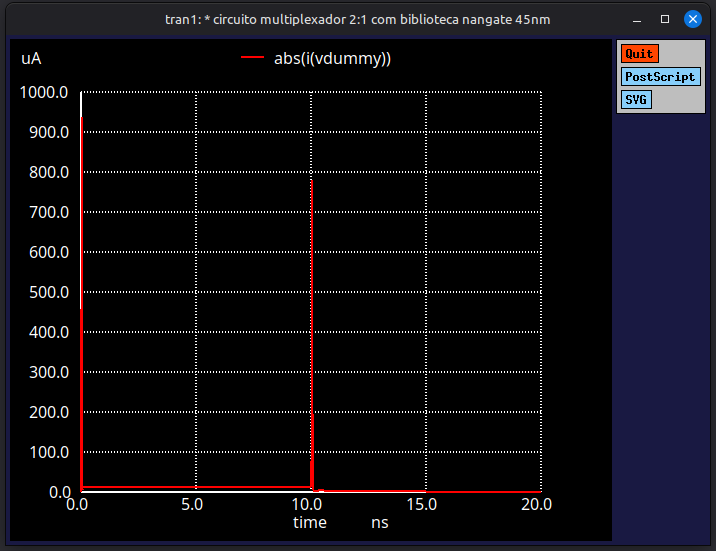
\includegraphics[width=\columnwidth]{3.png}}
\caption{Corrente drenada do circuito utilizando células com capacidade de fornecimento dobrada (X2).}
\label{fig3}
\end{figure}

\subsection{Células Complexas e Consumo Estático (Hora Trabalho)}
Avaliando a documentação da biblioteca Nangate e comparando a célula complexa de arranjo And-Or-Invert (\texttt{AOI21\_X1}) com a sua construção discreta feita utilizando um bloco de \texttt{AND2\_X1}, um \texttt{OR2\_X1} e um \texttt{INV\_X1}, observa-se uma discrepância favorável para a célula complexa.

O consumo estático (\textit{Leakage}) da célula integrada \texttt{AOI21\_X1} é significativamente inferior à soma dos consumos (leakages) independentes das três células primárias operando em conjunto. O motivo da discrepância reside na otimização em nível de silício (leiaute). Numa célula complexa do tipo AOI, os transistores compartilham intensamente poços (wells) e implantes de difusão, minimizando as fronteiras parasitas (junções). Isso não apenas economiza área física valiosa no \textit{die}, como elimina conexões metálicas intermediárias, reduzindo o número total de caminhos (junctions) pelos quais a corrente de fuga pode escapar ao substrato, tornando-a muito mais eficiente que a versão em portas separadas.

\section{Conclusões}
O Laboratório 05 evidenciou o impacto das decisões de engenharia num fluxo de projeto baseado em \textit{Standard Cells}. O simulador NGSpice mostrou de modo claro e mensurável que o uso de portas com um maior \textit{drive strength} (força motriz) só deve ser aplicado quando houver estrita necessidade de temporização de cargas pesadas, pois acarreta num forte aumento indesejado na potência dissipada dinamicamente pelo \textit{die}, conforme medido entre as instâncias 1X e 2X do MUX. 

Para a síntese de lógica combinacional otimizada, é constatado que projetistas lógicos não devem construir sistemas unicamente com blocos fundamentais simples. Utilizar blocos lógicos complexos encapsulados a nível de manufatura, como as portas AOI, oferece um tremendo benefício termodinâmico, garantindo a mesma tabela verdade teórica com uma resposta temporal mais homogênea e um consumo estático (fuga de corrente em repouso) brutalmente mitigado pela partilha física das regiões do semicondutor.

\begin{thebibliography}{00}
\bibitem{b1} R. A. L. Reis, \textit{Concepção de Circuitos Integrados}. Porto Alegre: Bookman, 2009.
\bibitem{b2} J. P. Uyemura, \textit{Sistemas digitais: uma abordagem integrada}. São Paulo: Thomson/Pioneira, 2002.
\bibitem{b3} R. Tocci, N. Widmer, and G. Moss, \textit{Sistemas Digitais - Princípios e Aplicações}, 12th ed. São Paulo: Pearson, 2018.
\end{thebibliography}

\end{document}